\chapter{Referencial Teórico}
\label{cap:REFERENCIAL}
No capitulo que segue será descrito o referencial teórico que serve de base para o desenvolvimento do estudo, além de trabalhos relacionados a área de análise de sentimentos e suas contribuições.
% falar de cada sessao criada nesse capitulo como guia

\section{Análise de Sentimentos}

A análise de sentimentos ou ainda, mineração de opinião é uma subárea da mineração de textos que analisa atitudes e emoções das pessoas sobre determinado tema. Ainda, segundo \citeonline{BAHRI2018669}, a análise de sentimentos tem por objetivo a classificação de um dado textual baseado no seu teor sentimental, de opinião, de avaliação e de atitudes, sendo útil na avaliação de determinadas entidades que podem ser eventos, produtos, problemas e etc. 

Tendo em vista o crescimento do número de usuários nas redes sociais, consequentemente o número de produções textuais nesses canais, e o interesse de grandes empresas em obter pesquisas de opinião de forma não invasiva e barata, ficou evidente que a analise de sentimento de forma manual realizada por especialistas tornou-se inviável sendo necessário o uso de recursos computacionais unidos a algoritmos sofisticados realizando analises em grande escala em menor tempo.
% falar sobre a procura pelas

\section{Etapas da Análise de Sentimentos}

Serão apresentadas as etapas principais para o processo de análise de sentimentos realizada de forma automática usando recursos computacionais para a sua execução.

\subsection{Coleta de Dados}
\label{subsec:coletadados}
A primeira fase para a mineração de opinião é a coleta de dados que serão posteriormente processados. Segundo \citeonline{9788576089346}, "Dados são fatos coletados e normalmente armazenados. Informação é o dado analisado e com algum significado. O conhecimento é a informação interpretada, entendida e aplicada para um fim.". O trabalho considerará dados eletrônicos digitais, mais precisamente, dados não estruturados (postagens textuais) gerados em redes sociais de forma manual. A informação principal considerada será a análise léxica baseada em categorias de emoções. Já o conhecimento pretendido será a aplicação estatística em cima das informações obtidas.

Para a fase de coleta de dados é importante primeiramente definir qual será a fonte de dados e, após, desenvolver ferramentas automáticas para a coleta dos dados que se pretende analisar futuramente. Algumas redes sociais disponibilizam APIs (\textit{Application Programming Interface}) para que aplicações sejam desenvolvidas usando o banco de dados dessas plataformas, permitindo tanto o consumo como a geração de dados dentro delas por meio de postagens de fotos, vídeos, textos. Essas ferramentas conseguem realizar buscas com filtros de data, usuários, palavras-chave, e etc. Sendo possível buscar amostras específicas conforme o que se queira pesquisar.

Geralmente as APIs são \textit{web services} (produtos disponibilizados na internet) baseados no protocolo HTTP (\textit{Hypertext Transfer Protocol}) e tornam os acessos seguros por meio da geração de \textit{tokens} a cada nova solicitação de inserção, alteração ou exclusão de dados. Um exemplo é a \textit{Graph API}\footnote{https://developers.facebook.com/docs/graph-api} desenvolvida pelo \textit{Facebook}, ela disponibiliza uma interface gráfica chamada \textit{Graph API Explorer} que pode ser vista na figura \ref{fig:GraphAPIExplorer}. A ferramenta é gratuita e tutoriais são disponibilizados para a aprendizagem.

\begin{figure}[!h]
\centering 
\caption{Tela do \textit{Graph API Explorer}}
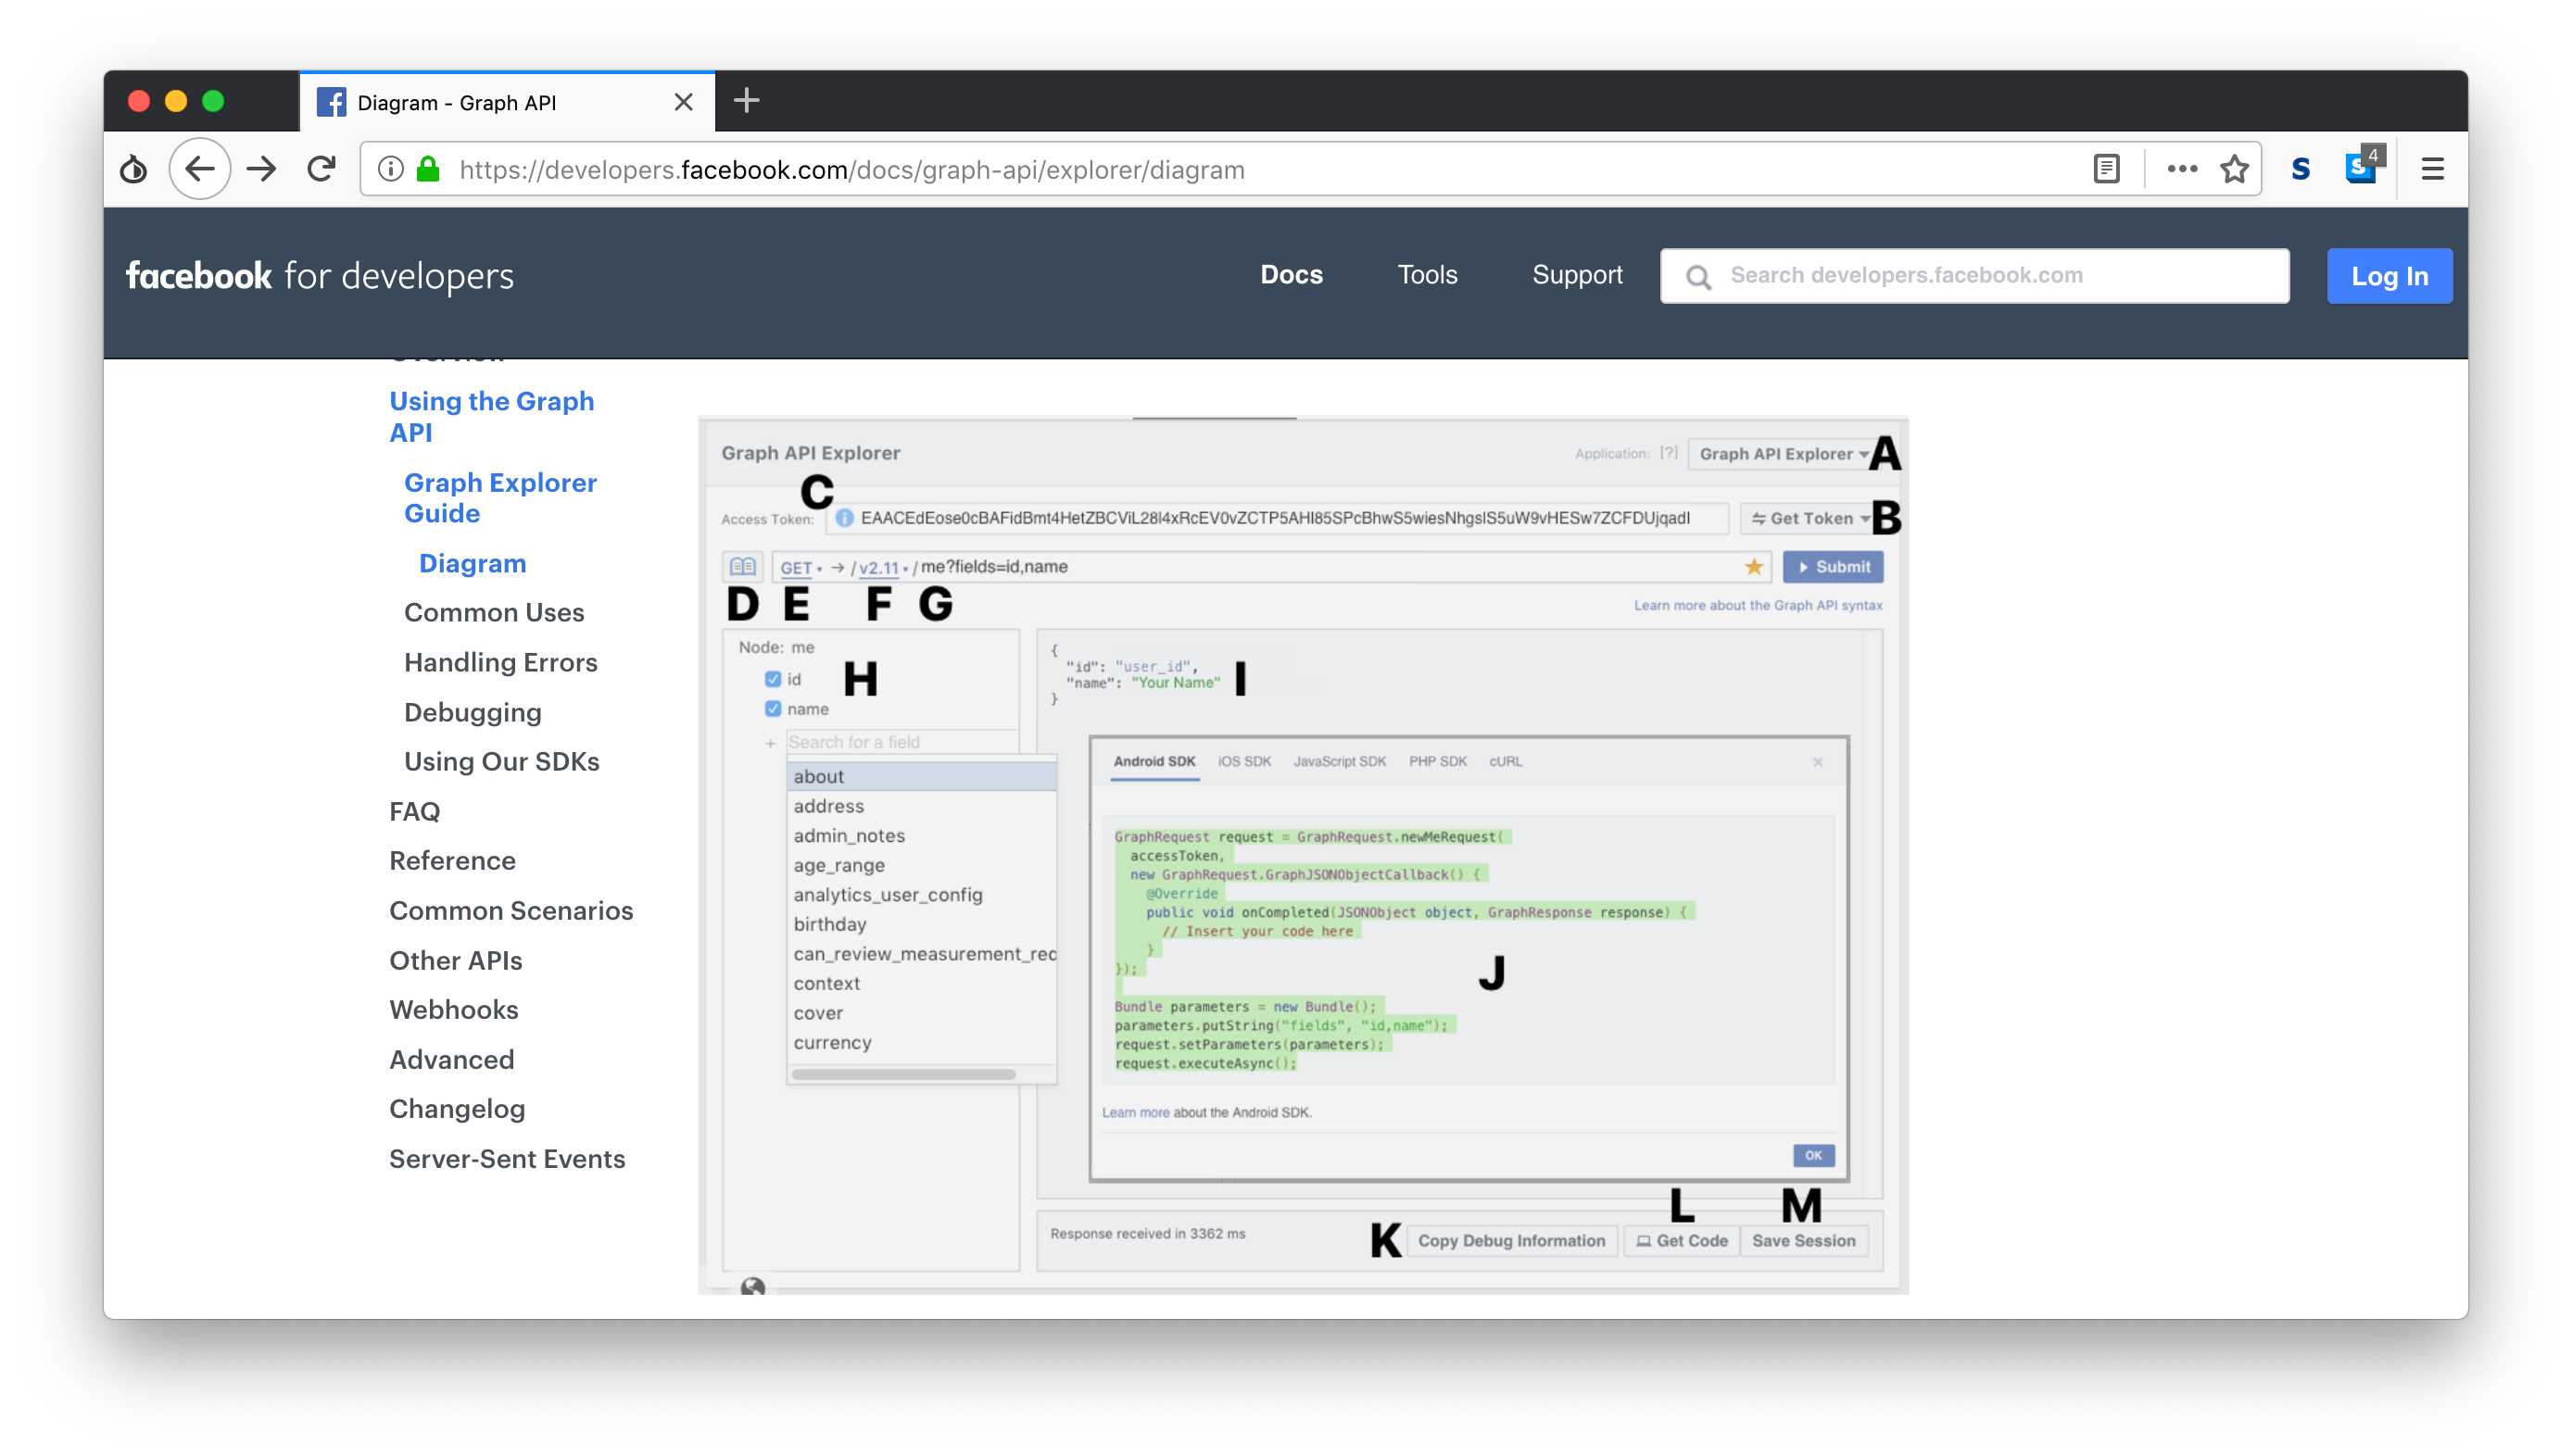
\includegraphics[scale=0.35]{imagens/graphapiexplorer.png}
\legend{Fonte: Facebook}
\label{fig:GraphAPIExplorer}
\end{figure}

\subsection{Pré-processamento dos Dados}
\label{subsec:preproc}

Após a coleta e armazenagem dos dados, é necessário a remoção de informações desnecessárias, a padronização do formato dos dados obtidos e a apresentação dos dados que serão, posteriormente, processados pelos algoritmos de extração de conhecimento. O pré-processamento inicia com a separação das frases em listas de palavras agora chamadas de \textit{tokens} que serão processadas até transformar o conteúdo inicial em sua forma reduzida e otimizada.\cite{SYMEONIDIS2018298}. É importante considerar que as técnicas de pré-processamento são utilizadas conforme a fonte de dados e também dos termos de interesse que serão buscados, assim como o idioma dos textos que se quer analisar. 

A seguir serão apresentadas as principais técnicas de pré-processamento textual conforme levantado pelos autores \citeonline{SYMEONIDIS2018298} sendo apresentadas em ordem de importância para um melhor resultado, tendo ganho de performance já que é possível a execução em paralelo entre as combinações de algumas técnicas.Também são citados alguns trabalhos que tratam cada uma das técnicas descritas.

\begin{itemize}
\item Remoção de \textit{unicode} e ruídos: Como nem todos os \textit{datasets} tem um tratamento prévio disponibilizado pelas ferramentas de coleta, é necessário um primeiro tratamento do seu conteúdo. Essa tarefa consiste em remover códigos \textit{unicode}\footnote{ Padrão internacional de códigos que permite que qualquer computador seja capaz de interpretar qualquer sistema de escrita\cite{0321480910}.} indesejados   como "\textbackslash u002c" e "\textbackslash x06". Essa é a primeira tarefa e também o ponto de partida para as demais tarefas de pré-processamento \cite{SYMEONIDIS2018298}.

\item Substituição de \textit{URL} e menções de usuários: A maioria dos conteúdos textuais em redes sociais contém \textit{URLs}, menções de usuário e \textit{tags} (sendo chamadas no \textit{Twitter} de \textit{hashtag}). Como esses conteúdos não apresentam nenhum conteúdo semântico e não expressam nenhum sentimento essa etapa tem por objetivo a remoção total ou substituição por um \textit{token} universal dentro do universo possível \cite{Khan2014}.
\label{it:giria}

\item Substituição de abreviaturas e gírias: Os usuários de redes sociais escrevem em linguagem informal e é comum o uso de gírias e de abreviação. Nessa etapa é gerada, manualmente, uma lista com as principais abreviaturas e expressões que se deseja detectar e também os termos que devem substituir essas frases. Assim, sempre que alguma frase especificada na lista for detectada, imediatamente será substituída pela frase equivalente \cite{Kouloumpis}.

\item Remoção de conteúdo numérico: Nessa etapa qualquer conteúdo numérico será removido pois eles não tem nenhum sentimento expresso. é importante a execução dessa etapa logo após a execução da tarefa \ref{it:giria} pois muitas gírias são compostas por números e a sua substituição já elimina a necessidade de remoção dos números \cite{He:2011:AEP:2002472.2002489}.

\item Substituição de pontuação repetida: Em muitos casos casos os usuários das redes sociais usam pontuações sendo eles de interrogação, de exclamação e de parada (ponto final) quando usados repetidamente significam sentimento intenso. Nessa etapa quando essas pontuações forem encontradas mais de uma vez em sequência as mesmas poderão ser substituídas por uma \textit{token} de mesmo valor em sentimento.

\item Remoção de pontuações: Sendo uma técnica muito comum na mineração de texto, essa consiste em remover as pontuações presentes no texto. Muitas literaturas afirmam que uma pontuação exclamativa pode significar um sentimento intenso positivo ou negativo e que sua remoção pode também alterar a acurácia da classificação do texto \cite{Lin2009}.

\item Manipulação de palavras em caixa alta: Palavras escritas em caixa alta são consideradas intensas de emoção. Por isso antes de padronizar todas as letras que compõem o texto para letras minúsculas, as palavras, com mais de duas letras, que forem escritas em caixa alta serão detectadas e sinalizadas para posterior processamento dos algoritmos de classificação .

\item Padronização de letras minúsculas: É a etapa mais comum verificada nas literaturas relacionas ao pré-processamento de texto. A etapa tem por objetivo a substituição de todos os caracteres maiúsculos para minúsculos, padronizando o conteúdo e facilitando as próximas etapas de pré-processamento \cite{DBLP:conf/coling/SantosG14}.

\item Remoção de \textit{stopwords}: Por definição, \textit{stopwords} são palavras de baixo peso e desnecessárias na análise de sentimento dos textos, são palavras com alta frequência de apresentação.  As \textit{stopwords} são adicionadas a listas chamadas por \textit{stoplists} previamente definidas conforme a necessidade da aplicação, podendo ser alterada a qualquer momento. Nessa etapa todas as palavras contidas na \textit{stoplist} serão removidas do texto já que não tem nenhuma utilidade na análise de sentimentos.

\item Substituição de palavras alongadas: As palavras alongadas são palavras escritas incorretamente com a repetição de algumas letras, escritas assim propositalmente para salientar sentimentos do autor. Nessa etapa as palavras alongadas serão encurtadas para sua forma original, perdendo parte do sentimento atribuído já que ocorrem com pouca frequência dentro de um mesmo texto \cite{Mohammad2015}.

\item Correção ortográfica: É comum em textos informais a presença de palavras com erros ortográficos. Nessa etapa é sugerido que, com o auxílio de dicionários externos ocorra uma correção ortográfica das palavras. Após a correção ortográfica a análise de sentimentos se torna mais simples já que as palavras incorretas trazem uma enorme dificuldade na classificação de sentimento das mesmas.

\item \textit{Part-of-Speech} (POS): Na etapa de POS, ou ainda, marcação de parte da fala, algumas classes de palavras são desconsideradas por não terem sentimentos atribuídos como advérbios, verbos, e etc. Na maioria dos estudos na área de pré-processamento de textos são considerados verbos, advérbios e substantivos, pois esses podem ser considerados na classificação \cite{Barbosa:2010:RSD:1944566.1944571}.

\item Lematização: Talvez uma das etapas mais complexas apresentadas nesse trabalho, tem por objetivo a busca dos lemas das palavras, isto é, fazer a análise morfológica das palavras em busca da remoção dos lexemas. Muitas literaturas não usam essa etapa pois a mesma é complexa e seu uso pode impactar na performance do pré-processamento \cite{Guzman2014}.

\item \textit{Stemming}: consiste na separação das palavras em \textit{radical} + \textit{terminação} para a análise apenas do radical das mesmas. Esse procedimento pode resultar em maior peso para o termo em posterior análise \cite{Porter1980}.
\end{itemize}

Após o pré-processamento, os dados estarão mais consistentes e padronizados, contendo as informações mais relevantes para a avaliação do conhecimento. Existem algumas tratativas específicas para \textit{emojis} e símbolos que também demonstram sentimento. Os mesmos não serão abordados no trabalho por ser de baixa relevância na pesquisa.

\subsection{Classificação dos Dados}
Após o pré-processamento, a próxima etapa da análise de sentimentos é a classificação dos dados. Atualmente existem vários estudos que buscam encontrar os métodos mais eficientes para a classificação, podendo ser visto na Figura \ref{fig:SAMethods} as principais abordagens para a etapa de classificação dos dados. Sendo que os algoritmos de \textit{Machine Learning} trazem um grande avanço na assertividade dos resultados da análise de sentimentos. Tradicionalmente os algoritmos de classificação de análise de sentimentos atribuem um sentimento como "positivo", "negativo" e "neutro", existindo algumas abordagens baseadas em análise de emoção que consideram categorias mais amplas baseadas no estudo de \citeonline{Ekman1992} que podem ser: alegria, tristeza, raiva, medo, nojo e surpresa.  

A seguir serão apresentados os principais métodos abordados nas literaturas referenciais que são os métodos baseados em léxico e os baseados em  aprendizado de máquina (\textit{machine learning}).

\begin{figure}[!h]
\centering 
\caption{Métodos de Classificação de SA}
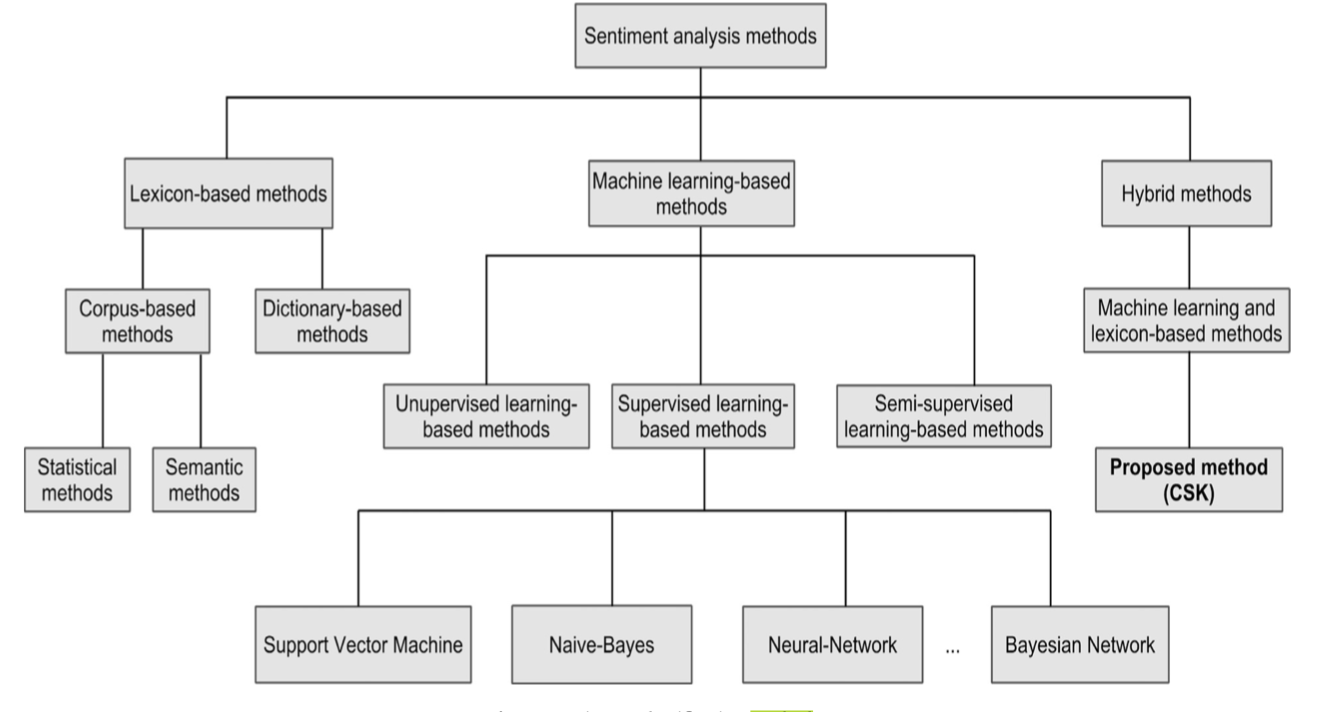
\includegraphics[scale=0.70]{imagens/sentimentanalysismethods.png}
\legend{Fonte: \citeauthor{CHANDRAPANDEY2017764}}
\label{fig:SAMethods}
\end{figure}
\newpage

\subsubsection{Método baseado em Aprendizado de Máquina}

Nessa abordagem a classificação dos dados ocorre com o auxilio de algoritmos de \textit{machine learning} como rede neural, algoritmo \textit{Naive-Bayes}, K-means e etc, podendo ser um algoritmo supervisionado, ou ainda, não-supervisionado. A seguir uma descrição e exemplos de cada abordagem.


\subsubsubsection{Métodos Supervisionados}

Segundo \citeonline{TRUYENS2014153}, são métodos supervisionados todos aqueles que usam exemplos fornecidos por especialistas humanos de domínio para ensinar o algoritmo a interpretar informações linguísticas interpretativas, ou seja, são algoritmos que tem uma fase de aprendizado \textit{a priori} de executar a classificação. Ainda segundo os autores, os algoritmos supervisionados geram resultados significantes porém, têm um algo custo devido ao esforço humano necessário. Mesmo assim, algumas práticas semi-supervisionadas, usando uma pequena base de dados rotulados e conjunto a uma base maior não rotulada relacionadas por suposição (por exemplo, pela distribuição uniforme dos dados) os resultados são realmente satisfatórios \cite{TRUYENS2014153}.

O principal algoritmo supervisionado utilizado dentro da classificação de sentimentos é o \textit{Naive Bayes} (NB) por unir simplicidade e eficiência nos cenários mais diversos, especialmente quando aplicado a um conjunto de dados onde seus atributos são independentes \cite{VIEGAS2018153}. 

O Naive Bayes é um algoritmo probabilístico baseado no Teorema de Bayes representado na Equação \ref{eq:naivebayes}. Ela é definida como "a probabilidade de A dado B", ou seja, qual a probabilidade de A estar dentro de um conjunto de evidências assumido como B \cite{schmitt2013analise}.

\begin{equation}
    \label{eq:naivebayes}
     P\left ( A| B \right ) = \frac{P\left ( B|A \right )P\left ( A \right )}{P\left ( B \right )}
\end{equation}

O algoritmo é considerado ingênuo (\textit{naive}) por assumir que cada atributo é independente, ou seja, a informação de um evento não é informativa sobre nenhum outro. A Figura \ref{fig:ModeloNaiveBayes}  indica que cada atributo $A_{i}$ influência a classe $C$ unicamente sem nenhum atributo influenciar qualquer outro \cite{schmitt2013analise}.

\begin{figure}[!h]
\centering 
\caption{Modelo Naive Bayes}
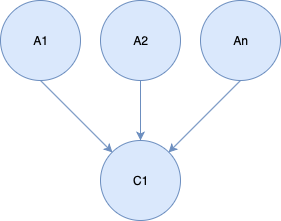
\includegraphics[scale=0.70]{imagens/modeloNaiveBayes.png}
\legend{Fonte: O autor baseado em \citeauthor{schmitt2013analise}}
\label{fig:ModeloNaiveBayes}
\end{figure}

O algoritmo pode ser usado de forma incremental conforme a necessidade de sua revisão probabilística. Existem varias abordagens de modelo sendo os principais o modelo binário e o modelo multidimensional. No modelo binário, cada documento é representado por um vetor binário onde a a presença ou a ausência de um termo é representado, respectivamente, por $1$ e $0$. Já no modelo multidimensional a representação ocorre por vetores de números inteiros por documento, onde  cada índice do vetor representa a quantidade de vezes que um termo acontece no documento \cite{schmitt2013analise}.

\subsubsubsection {Métodos Não-Supervisionados} 

São tidos como métodos não-supervisionados aqueles que o próprio algoritmo - sem o auxilio de aprendizado a partir de treinamento - determina as características do texto. Um exemplo é a clusterização de textos onde o software analisa um conteúdo textual encontrando, independentemente, grupos de palavras com similaridade entre elas. Essa abordagem é baseada em três etapas principais: a medida de proximidade, estratégia de agrupamento e seleção de descritores.

Na etapa de medida de proximidade verifica-se a similaridade entre os textos, dependendo da abordagem também é válido buscar a dissimilaridade entre os textos. Os dois métodos mais conhecidos para a obtenção dessa medida de proximidade para dados do tipo texto são os métodos: Cosseno e Jaccard. Para a execução de ambos os métodos é necessário considerar dois vetores documentos $x_{i}=\left ( x_{i1}, x_{i2}, \dotsc, x_{im}\right )$ e $x_{j}=\left ( x_{j1}, x_{j2}, \dotsc, x_{jm}\right )$ onde cada termo da coleção é representado em uma das dimensões dos vetores \cite{Rezende2011}.

O método do cosseno, expresso na Fórmula \ref{eq:cosseno}, define a semelhança dos termos conforme o ângulo que os vetores formam entre si. Para ângulos próximos de $90^{\circ}$, ou seja, cosseno próximo de 0, os documentos não compartilham nenhum termo. Já para ângulos próximos de $0^{\circ}$, e  cosseno próximo de 1, os documentos têm termos semelhantes \cite{Rezende2011}.

\begin{equation}
    \label{eq:cosseno}
     \cos \left ( x_{i},x_{j} \right ) = \frac{\sum_{l=1}^{m} x_{il} x_{jl}}{\sqrt{\sum_{l=1}^{m} x_{il^{2}} \sum_{l=1}^{m} x_{jl^{2}}} }
\end{equation}

Para as situações em que os vetores são representados por valores binários, indicando presença ou ausência de determinados termos, o cálculo de proximidade pode ser realizado pelo método Jaccard \cite{Rezende2011}.

Para o cálculo considera-se os mesmos vetores $x_{i}$ e $x_{j}$  considerando também as seguintes contagens:

$f_{01}$: Número de termos ausentes em $x_{i}$ e presentes em $x_{j}$;

$f_{10}$: Número de termos presentes em $x_{i}$ e ausentes em $x_{j}$;

$f_{11}$: Número de termos presentes em ambos os vetores.

Com essas medidas, a medida jaccard é dada conforme a Fórmula \ref{eq:jaccard}. O resultado estará compreendido entre $\left [ 0,1 \right ]$ sendo que quanto mais próximo de $1$, maior a similaridade dos termos.

\begin{equation}
    \label{eq:jaccard}
     jaccard(x_{i},x_{j}) = \frac{f_{11} }{f_{10} +f_{01}  + f_{11} }
\end{equation}

Após encontrar as medidas de similaridade é necessário  realizar a etapa de agrupamento sendo o \textit{k-means} um dos modos mais utilizados onde o objetivo é agrupar os vetores em $k$ grupos. A seguir são apresentadas as características do \textit{k-means} conforme  \citeonline{Steinbach00acomparison}.

O \textit{k-means} é baseado na ideia de que um ponto central pode representar um \textit{cluster}, nessa técnica se usa a noção de centroide que significa o ponto médio central de um grupo de pontos. Geralmente o centroide é um ponto diferente de um ponto de dados real e é calculado a partir dos demais vetores do grupo \cite{Steinbach00acomparison}. A fórmula do centroide para um vetor de tamanho $G$, onde $x$ é um vetor documento é dada a seguir:

\begin{equation}
    \label{eq:centroide}
     C=\frac{1}{|G|}\sum_{x \in G}x
\end{equation}

Como entrada do algoritmo \textit{k-means} tem-se um conjunto de vetores documento e $k$ que é o número referente a quantidade de grupos que se deseja se dividam. A partir daí o algoritmo selecionará $k$ vetores aleatórios como centroides iniciais e repetir o calculo de dissimilaridade de cada vetor para cada centroide e inserir o documento no grupo no qual ele mais se assemelha, após, uma nova centroide será calculada tendo em vista os vetores que foram adicionados a ele. O algoritmo pode assumir duas regras de parada: na primeira, é considerado o número de iterações e na segunda é considerado a situação onde não ocorrem mais alterações nos vetores, ou seja, os vetores não trocarem mais de grupos \cite{Steinbach00acomparison}.

A última etapa dos métodos não-supervisionados é a seleção de descritores para apresentação dos resultados para a próxima etapa da análise de sentimentos. Alguns métodos para a seleção de descritores utilizam o centroide já que ele mantém a característica central de todos os grupos.

\subsubsection{Método baseado em léxico}
\label{subsubsec:lexico}
No método baseado em léxico o sentimento (polaridade) é calculado conforme sua orientação semântica. É necessário definir um dicionário léxico com as polaridades correspondentes de cada palavra que o compõe. Esses dicionários podem ser criados manualmente ou automaticamente usando radicais de palavras e as adicionando a lista conforme apresentado por \citeauthor{Taboada}. Primeiro uma lista de adjetivos e suas polaridades correspondentes é desenvolvida e um dicionário é criado. Após, quando um texto for analisado todos os seus adjetivos serão extraídos e arquivados junto de seus valores que podem no final gerar uma polaridade única do texto analisado \cite{Taboada}.Existem duas subclasses principais dentro da abordagem léxica que são: as técnicas de análise de sentimento baseadas em dicionário e as técnicas de análise de sentimento baseada em corpo \cite{LIU2017149}.

Na AS baseada em dicionário o foco principal da técnica é a construção de dicionários de sentimento, onde um pequeno conjunto de palavras e sentimentos é determinado manualmente e após ocorre uma pesquisa dos antônimos e sinônimos nas corporas mais populares como o \textit{WordNet} \cite{Miller:1995:WLD:219717.219748}, \textit{HowNet}, ou ainda \textit{Thesaurus}, fazendo com que novas palavras sejam encontradas e o dicionário aumente consideravelmente. No processo iterativo da técnica é realizado até que nenhuma nova palavra possa ser encontrada resultando em um dicionário de sentimentos \cite{LIU2017149}. 

Já na AS baseada em corpo é comumente utilizada quando quando se quer encontrar padrões sintáticos de contextos específicos. O foco da técnica é encontrar os padrões sintáticos e uma lista de radicais, comumente chamados de sementes, de palavras de opinião. Para chegar ao resultado, a técnica usa técnicas estatísticas para encontrar as palavras sementes enquanto as técnicas semânticas são utilizadas para determinar os valores semânticos para as palavras conforme a similaridade conforme as diferentes palavras \cite{LIU2017149}.

\section{Redes Sociais}
\label{sec:RedesSociais}
Desde o princípio, a humanidade tem a necessidade de conviver em comunidade, sendo necessário a vida em conjunto na realização de trabalhos como também para a formação de famílias e grupos. Esses grupos eram formados conforme afinidades políticas, religiosas, étnicas, profissionais e etc, trazendo como resultado o constante desenvolvimento social e e intelectual do homem até os dias atuais \cite{KHALED2018}. Com o desenvolvimento da internet esse comportamento também foi replicado para a rede em plataformas denominadas \textit{Online Social Network} (OSN), também chamadas de Redes Sociais, que segundo \citeonline{N2018777} vão além de plataformas de comunicação e troca de informações, mas também chegam a impactar no crescimento econômico. 

São exemplos de redes sociais o \textit{Facebook}\footnote{https://www.facebook.com}, o \textit{Twitter}\footnote{https://twitter.com} e o \textit{Instagram}\footnote{https://www.instagram.com} sendo todos baseados na cocriação com o usuário, isto é, ele que gera o conteúdo das plataformas através dos seus \textit{posts}, as conexões através das solicitações de conexão com outro usuário, comunidades através de páginas de afinidade e grupos, e sinaliza possíveis melhorias para as plataformas seguirem em contínua evolução atraindo mais usuários a cada ano como pode ser visto na Tabela \ref{tab:qtdusers} a quantidade de usuários em Agosto de 2018 nas redes sociais.


\begin{table}[h]
\centering
\caption{Quantidade de Usuários nas Redes Sociais}
\label{tab:qtdusers}
\begin{tabular}{|l|c|}
\hline
\textbf{Rede Social}&  \textbf{Número de Usuários} \\ \hline
Facebook     &     2.23 bilhões   \\ \hline
Youtube      &     1.9  bilhão    \\ \hline
Instagram    &     1    bilhão    \\ \hline
Twitter      &     336  milhões   \\ \hline
Reddit       &     330  milhões    \\ \hline
Pinterest    &     200  milhões    \\ \hline
Ask.fm       &     160  milhões    \\ \hline
\end{tabular}
\legend{Fonte: \citeauthor{kallas_2018}}
\end{table}

Existem redes sociais com o foco em conteúdo visual, que é o caso do \textit{Instagram}, rede social fundada em 6 de Outubro de 2010 por Kevin Systrom (CEO e co-fundador) e Mike Krieger (CTO e co-fundador) que revolucionou a forma de compartilhar fotos. Segundo Kevin Systrom o \textit{Instagram} se tornou o lar das narrativas visuais sendo possível que artistas, músicos, celebridades e qualquer tipo de pessoa compartilhe seus conteúdos \cite{instagram_2018}. A rede social conta com mais de 400 milhões de novas postagens na categoria de \textit{Story} diariamente. 

Também é o caso do \textit{Snapchat}, em que a companhia se intitula como uma \textit{empresa de câmeras} e que acredita que a revolução da sua ferramenta contribui com a forma das pessoas se expressarem, aprenderem sobre o mundo e se divertirem juntas \cite{snapchat_2018}. No Snapchat as pessoas podem compartilhar momentos instantâneos por meio de foto ou video, fazendo edições rápidas e casuais podendo também temporizar o tempo de exibição das postagens conforme necessitar.

O foco do trabalho desenvolvido é em redes sociais com conteúdo textual, como é o exemplo do \textit{Facebook} e o \textit{Twitter} já que serão utilizados os métodos de pré-processamento abordados na sub-sessão \ref{subsec:preproc} afim de melhorar a detecção de sentimentos. Dessa forma redes sociais com conteúdo de imagem como é caso do \textit{Instagram} podem ser avaliadas por trabalhos futuros com outras abordagens de pré-processamento e detecção de sentimentos.

\section{Revisão de Ferramenta Implementada}
\label{sec:revisaoferramenta}
Com o crescimento das pesquisas no campo da mineração de texto e com as variadas aplicações encontradas para a análise de sentimentos, cada vez mais ferramentas são desenvolvidas com os mais variados propósitos de pesquisa e também para aplicações comerciais. A ferramenta base para o trabalho aqui desenvolvido é resultado de uma pesquisa realizada por \citeonline{tccfilipe} que resultou em um software \textit{web crawler}\footnote{ \textit{Softwares} que criam conexão com determinado \textit{site} e extraem informações desejadas por meio de APIs geralmente disponibilizadas pelo meio eletrônico.} que realiza a análise de sentimentos em uma interface relativamente simples para usuários que não têm experiência em programação.

É possível verificar na Figura \ref{fig:fluxotccfilipe} o fluxo de funcionalidades da ferramenta implementada onde, inicialmente, o usuário entra com uma URL de busca e a quantidade de postagens a ser analisada (Figura \ref{fig:menutccfilipe}) e após ocorre a classificação e por fim ocorre a apresentação das informações em forma de nuvem de palavras (Figura \ref{fig:nuvemtccfilipe}), gráficos (Figura \ref{fig:graficotccfilipe}), e ainda, em relatórios gerados em PDF (Figura \ref{fig:exportadotccfilipe}). A coleta de dados ocorreu com a API apresentada na sub-sessão \ref{subsec:coletadados} chamada \textit{Facebook Graph API}, a partir dela o \textit{software} faz buscas na rede social \textit{Facebook} e coleta postagens conforme parametrizado.

\newpage

\begin{figure}[!h]
\centering 
\caption{Fluxograma de funcionalidades do software revisado}
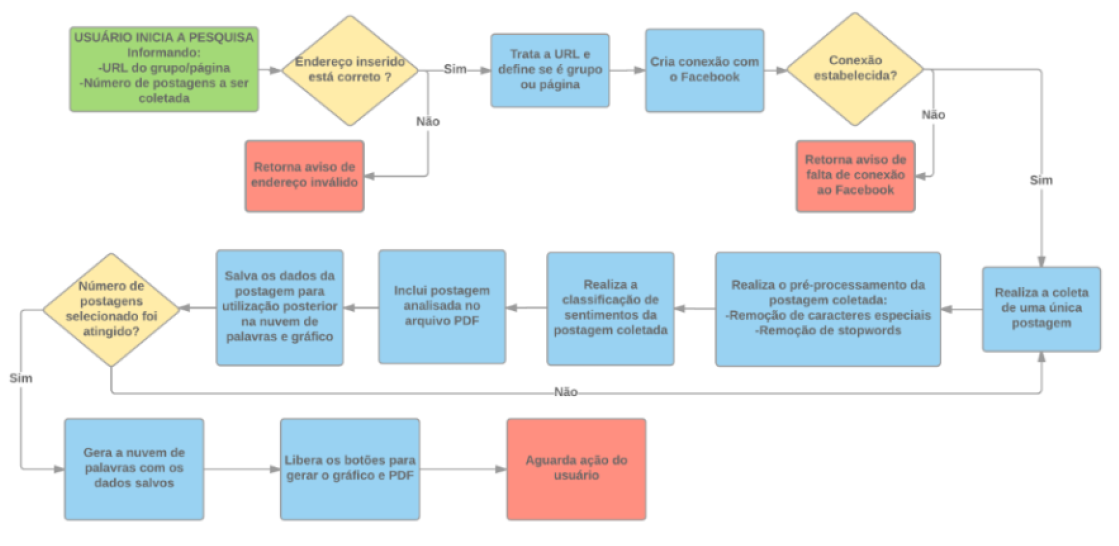
\includegraphics[scale=0.46]{imagens/fluxofilipe.png}
\legend{Fonte: \citeauthor{tccfilipe}}
\label{fig:fluxotccfilipe}
\end{figure}

\begin{figure}[!h]
\centering 
\caption{Menu de busca do software revisado}
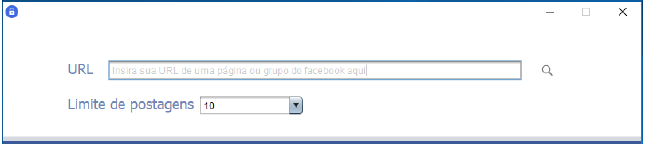
\includegraphics[scale=0.5]{imagens/menudebuscafilipe.png}
\legend{Fonte: \citeauthor{tccfilipe}}
\label{fig:menutccfilipe}
\end{figure}

\begin{figure}[!h]
\centering 
\caption{Nuvem de palavras do software revisado}
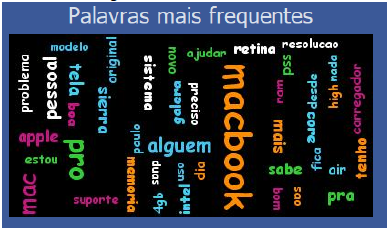
\includegraphics[scale=0.62]{imagens/nuvemdepalavras.png}
\legend{Fonte: \citeauthor{tccfilipe}}
\label{fig:nuvemtccfilipe}
\end{figure}

\begin{figure}[!h]
\centering 
\caption{Gráfico de sentimentos do software revisado}
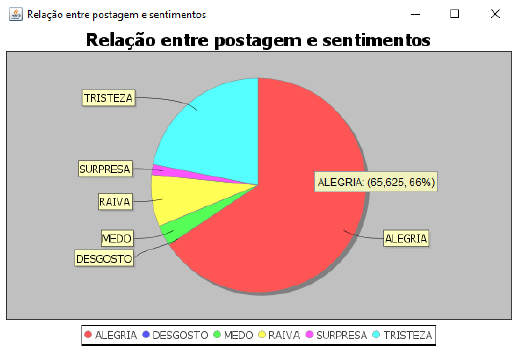
\includegraphics[scale=0.8]{imagens/graficodesentimentosfilipe.png}
\legend{Fonte: \citeauthor{tccfilipe}}
\label{fig:graficotccfilipe}
\end{figure}

\begin{figure}[!h]
\centering 
\caption{Resultado exportado do software revisado}
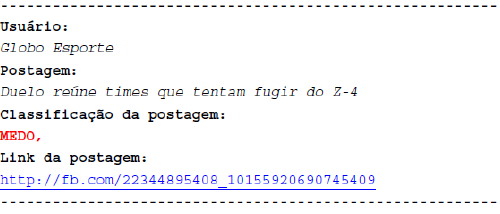
\includegraphics[scale=0.60]{imagens/exportadofilipe.png}
\legend{Fonte: \citeauthor{tccfilipe}}
\label{fig:exportadotccfilipe}
\end{figure}

\newpage
Para atingir o propósito de sua pesquisa, \citeauthor{tccfilipe} realizou o estudo de léxicos de emoções contidos na base de dados chamada \textit{WordNet}\footnote{https://wordnet.princeton.edu} categorizados em seis grupos distintos que foram: alegria, desgosto, medo, raiva, surpresa e tristeza. Na Tabela \ref{tab:categoriaemo} estão alguns exemplos de palavras separadas pelas respectivas categorias de emoção selecionado pelo autor. Além da análise de sentimentos também foi implementada busca por palavras frequentemente encontradas em ataques de \textit{phishing},  e também palavras de linguagem imprópria, visto que as redes sociais não mantém um filtro de conteúdo levando em consideração a idade do usuário.

\begin{table}[h!]
  \begin{center}
    \caption{Categorias de emoções}
    \label{tab:categoriaemo}
    \begin{tabular}{ll} % <-- Alignments: 1st column left, 2nd middle and 3rd right, with vertical lines in between
      \textbf{Categoria} & \textbf{Palavras}\\
      \hline
      Alegria&animação, ânimo, comédia\\
      Desgosto&maldoso, chatear, abominável\\
      Medo&desespero, escuridão, friamente\\
      Raiva&assassinar, bravejar, detestar\\
      Surpresa&chocante, espanto, impressionado\\
      Tristeza&cabisbaixo, chorão, culpa\\
      \hline
    \end{tabular}
  \end{center}
  \legend{Fonte: \citeauthor{tccfilipe}}
\end{table}
Após definir os grupos de coleta, os dados de coleta para a análise de sentimentos e realizar a classificação dos dados utilizando método de classificação baseado em léxicos, o autor realizou a análise dos resultados para constatar o quão precisa foi a classificação realizada pela ferramenta. \citeauthor{tccfilipe} coletou amostras de diferentes tamanhos em todos os grupos analisados totalizando 50 (cinquenta), 100 (cem) e 500 (quinhentos) postagens para, após, serem também analisadas manualmente e assim comparar os resultados. Dentre os grupos estudados estão a página do \textit{Outback Brasil} e o grupo da Previdência Social, alguns ajustes de léxicos foram necessários para que as classificações ocorressem com maior assertividade nos casos de alegria e tristeza. No final foi realizada a comparação entre as classificações e exatificadas as suas respectivas taxas de acerto, a Tabela \ref{tab:taxaacerto} apresenta os resultados obtidos, com eles foi possível verificar que quatro dos sentimentos tiveram taxa de acerto superiores a oitenta por cento. Com o cálculo do desvio padrão foi possível constatar que nos sentimentos com menor classificação refletiam uma grande dispersão em torno da media populacional, resultado de expressões ambíguas e de duplo sentido.

\begin{table}[h!]
  \begin{center}
    \caption{Taxa média de acerto na classificação de postagens analisadas}
    \label{tab:taxaacerto}
    \begin{tabular}{lllllll} % <-- Alignments: 1st column left, 2nd middle and 3rd right, with vertical lines in between
      \textbf{Classificação} & \textbf{Alegria} & \textbf{Medo} & \textbf{Tristeza} & \textbf{Desgosto} & \textbf{Raiva} & \textbf{Surpresa}\\
      \hline
      Taxa de Acerto&52,82\%&90,77\%&81,55\%&88,89\%&91,01\%&75,83\%\\
      Desvio Padrão($\sigma$)&16,06&2,62&5,20&4,61&4,23&9,97\\
      \hline
    \end{tabular}
  \end{center}
  \legend{Fonte: \citeauthor{tccfilipe}}
\end{table}

Ao final dos estudos foi concluído que a ferramenta desenvolvida trouxe resultados satisfatórios tanto pelos resultados obtidos como pela facilidade que a ferramenta desenvolvida trás para os usuários comuns. Ainda, foram apontadas melhorias para os estudos futuros entre elas o desenvolvimento de uma plataforma \textit{web}, aprimoramento nos testes de resultados da análise de sentimentos e também novas abordagens na etapa de classificação dos dados. 

% falar aqui sobre os resultados encontrados pelo filipe
% \section{Estado da Arte da Análise de Sentimentos}
% Nessa sub-sessão será apresentado o estado da arte da Análise de Sentimentos 

% Para realizar a pesquisa do estado da arte da análise de sentimentos baseada em emoções nas redes sociais foi utilizado a plataforma de pesquisa desenvolvida pela editora \textit{Elsevier} chamada de \textit{ScienceDirect} para assim obter acesso aos conteúdos mais conceituados sobre o assunto em estudo.

% \begin{figure}[!h]
% \centering 
% \caption{Mapa mental de expressões relevantes para pesquisa}
% 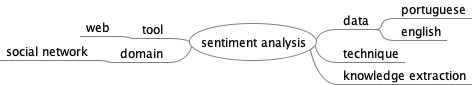
\includegraphics[scale=0.8]{imagens/mapamental.png}
% \legend{Fonte: O Autor}
% \label{fig:mapamentalautor}
% \end{figure}
% \section{Considerações Finais}
